%%
% Plantilla de Memoria
% Modificación de una plantilla de Latex de Nicolas Diaz para adaptarla 
% al castellano y a las necesidades de escribir informática y matemáticas.
%
% Editada por: Mario Román
%
% License:
% CC BY-NC-SA 3.0 (http://creativecommons.org/licenses/by-nc-sa/3.0/)
%%

%%%%%%%%%%%%%%%%%%%%%
% Thin Sectioned Essay
% LaTeX Template
% Version 1.0 (3/8/13)
%
% This template has been downloaded from:
% http://www.LaTeXTemplates.com
%
% Original Author:
% Nicolas Diaz (nsdiaz@uc.cl) with extensive modifications by:
% Vel (vel@latextemplates.com)
%
% License:
% CC BY-NC-SA 3.0 (http://creativecommons.org/licenses/by-nc-sa/3.0/)
%
%%%%%%%%%%%%%%%%%%%%%

%----------------------------------------------------------------------------------------
%	PAQUETES Y CONFIGURACIÓN DEL DOCUMENTO
%----------------------------------------------------------------------------------------

%% Configuración del papel.
% microtype: Tipografía.
% mathpazo: Usa la fuente Palatino.
\documentclass[a4paper, 11pt]{article}
\usepackage[protrusion=true,expansion=true]{microtype}
\usepackage{mathpazo}

% Indentación de párrafos para Palatino
\setlength{\parindent}{0pt}
  \parskip=8pt
\linespread{1.05} % Change line spacing here, Palatino benefits from a slight increase by default

% Enlaces
\usepackage[hidelinks]{hyperref}

%% Castellano.
% noquoting: Permite uso de comillas no españolas.
% lcroman: Permite la enumeración con numerales romanos en minúscula.
% fontenc: Usa la fuente completa para que pueda copiarse correctamente del pdf.
\usepackage[spanish,es-noquoting,es-lcroman]{babel}
\usepackage[utf8]{inputenc}
\usepackage[T1]{fontenc}
\selectlanguage{spanish}

%% Gráficos
\usepackage{graphics,graphicx, float, url} % Required for including pictures
\usepackage{wrapfig} % Allows in-line images
\usepackage[usenames,dvipsnames]{color} % Coloring code
\usepackage{caption}
\usepackage{subcaption}

% Para algoritmos
\usepackage{algorithm}
\usepackage{algorithmic}
\usepackage{amsthm}

\makeatletter

%----------------------------------------------------------------------------------------
%	TÍTULO
%----------------------------------------------------------------------------------------
% Configuraciones para el título.
% El título no debe editarse aquí.
\renewcommand{\maketitle}{
  \begin{flushright} % Right align
  
  {\LARGE\@title} % Increase the font size of the title
  
  \vspace{50pt} % Some vertical space between the title and author name
  
  {\large\@author} % Author name
  \\\@date % Date
  \vspace{40pt} % Some vertical space between the author block and abstract
  \end{flushright}
}

% Título
\title{\textbf{Prácticas PDDL: Planificación}\\ % Title
Entrega 1: Dominios y problemas de planificación clásica en PDDL} % Subtitle

\author{\textsc{Óscar Bermúdez Garrido} % Author
\\{\textit{Universidad de Granada}}} % Institution

\date{\today} % Date

%----------------------------------------------------------------------------------------
%	DOCUMENTO
%----------------------------------------------------------------------------------------

\begin{document}

\maketitle % Print the title section

% Resumen (Descomentar para usarlo)
\renewcommand{\abstractname}{Resumen} % Uncomment to change the name of the abstract to something else
\begin{abstract}
	En esta práctica, nos presentan una aventura gráfica y tenemos que modelar sus reglas, objetivos, así
	como el comportamiento del jugador de forma deliberativa para lograr alcanzar las metas que se le vayan
	proponiendo de la forma más óptima posible.
\end{abstract}

% Índice
{\parskip=2pt
  \tableofcontents
}
\pagebreak

%% Inicio del documento

\section{Mapa del mundo}
	Por la complejidad de las 25 zonas, me fue necesario el dibujo de un mapa para testear (que
	posteriormente reutilicé) para facilitarme la creación del archivo de problema y no dejar
	zonas aislada.
	
	Las posibles zonas aisladas se pueden producir por:
	\begin{itemize}
		\item Establecer dos o más zonas no conectadas.
		\item Ubicar precipios en zonas que necesitaban ser transitables.
		\item De forma más complicada, colocar bosques o agua en zonas que necesiten ser atravesadas
		sin colocar el objeto correspondiente para atravesarlos de forma accesible.
	\end{itemize} 
	
	El mapa utilizado fue el siguiente:
	\begin{figure}[H]
		\centering
		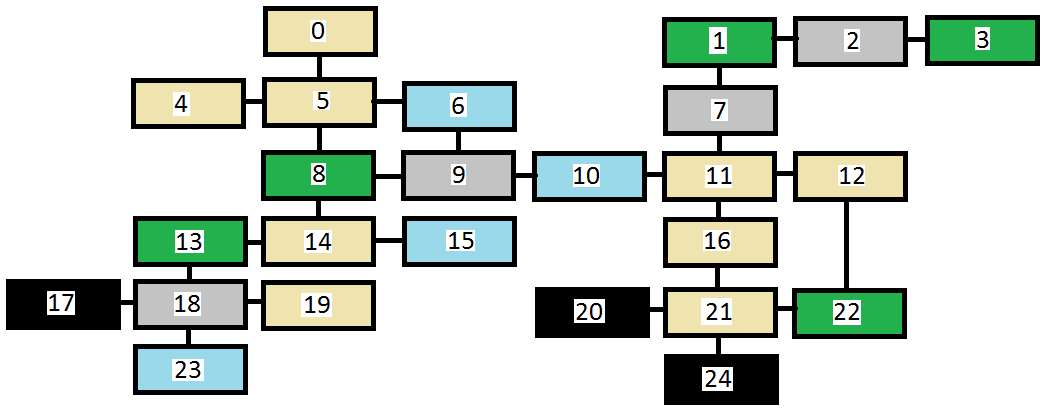
\includegraphics[width=15cm]{BelkanWorld.png}
		\caption{Mapa de los mundos de Belkan.}
		\label{world}
	\end{figure}
	
	La colocación del jugador, los personajes, los objetos y los tipos de terrenos fue arbitraria pero
	verificando que era posible el correcto paso por todas las zonas permitidas.

\section{Características básicas}
	En este apartado, se configuran las características más básicas del juego, dejando para apartados
	posteriores la implementación de las reglas, limitaciones y optimizaciones.
	
	\subsection{Objetos del mundo}
		Para la implementación de los objetos del mundo, usaremos la sintaxis de PDDL dada por:
		\begin{verbatim}
		(:types jugador
		        personaje
		        objeto
		        zona
		)
		\end{verbatim}
		
		Aunque se podría haber optado por definir cada uno de los personajes y objetos en este
		apartado, considero más adecuado la inicialización de los distintos personajes y objetos
		dentro del archivo de problema.
	
	\subsection{Estados del mundo}
		Para el correcto mantenimiento del mundo, debemos utilizar estados o predicados para comprobar
		el estado actual del mundo, permitiendo así conocer:
		\begin{itemize}
			\item Zonas que están conectadas mediante el predicado \textit{(conectada ?z1 ?z2 - zona)}
			\item La disponibilidad de objetos, así como la ubicación de los personajes o el propio
			jugador dentro del mapa que tenemos usando \textit{(at ?x - (either jugador personaje objeto)
			?z - zona)}.
			\item Si el jugador tiene algún objeto encima con \textit{(libre ?j - jugador)}.
			\item En caso de tener un objeto, cuál es comprobando \textit{(cogido ?o - objeto ?j -
			jugador)}.
			\item Y finalmente, qué objeto entregamos: \textit{(entregado ?o - objeto ?p - personaje)}.
		\end{itemize}

	\subsection{Acciones permitidas}
		Claramente, necesitamos definir unas instrucciones básicas para interactuar con el mundo:
		\begin{itemize}
			\item \textit{ir}: Esta acción nos permite mover al jugador de una zona a otra, por tanto,
			tenemos que comprobar que nuestro personaje está en la primera zona antes de movernos y que
			ambas zonas estén unidas para poder ir en un sólo paso, y el resultado será que el personaje
			está en la nueva zona y no en la primera como se puede apreciar:
			\begin{verbatim}
(:action ir
   :parameters (?j - jugador ?origen ?destino - zona)
   :precondition (and (at ?j ?origen)
                      (or
                         (conectada ?origen ?destino)
                         (conectada ?destino ?origen)
                      )
                 )
   :effect (and (at ?j ?destino)
                (not (at ?j ?origen))
           )
)
			\end{verbatim}
			
			\item \textit{coger}: Esta acción permite al jugador recoger un objeto del suelo, por tanto,
			tenemos que comprobar que nuestro personaje y el objeto que vamos a coger, están en la misma
			zona y que el jugador no tiene otro objeto ya, y el resultado será que el personaje coge el
			objeto y el objeto ya no está en la zona del mundo, como se comprueba en el código:
			\begin{verbatim}
(:action coger
   :parameters (?z - zona ?o - objeto ?j - jugador)
   :precondition (and (at ?o ?z)
                      (libre ?j)
                      (at ?j ?z)
                 )
   :effect (and (not (libre ?j))
                (cogido ?o ?j )
                (not (at ?o ?z))
           )
)
			\end{verbatim}

			\item \textit{coger}: Esta acción permite al jugador dejar un objeto en una zona, por tanto,
			tenemos que comprobar que nuestro personaje tiene el objeto cogido y que el jugador está en
			la zona en la que lo quiere soltar, y el resultado será que el personaje está libre y el
			objeto está en la zona del mundo indicada, como se refleja en la acción:
			\begin{verbatim}
(:action dejar
   :parameters (?z - zona ?o - objeto ?j - jugador)
   :precondition (and (cogido ?o ?j)
                      (at ?j ?z)
                 )
   :effect (and (at ?o ?z)
                (libre ?j)
                (not (cogido ?o ?j))
           )
)
			\end{verbatim}

			\item \textit{entregar}: Esta acción permite al jugador entregar un objeto a un personaje, por
			tanto, tenemos que comprobar que nuestro personaje y el personaje están en la misma zona y que
			el personaje tiene el objeto, y el resultado será que el personaje estará libre y que se ha
			entregado el objeto al personaje como podemos ver:
			\begin{verbatim}
(:action entregar
   :parameters (?z - zona ?o - objeto ?j - jugador ?p - personaje)
   :precondition (and (cogido ?o ?j)
                      (at ?j ?z)
                      (at ?p ?z)
                 )
   :effect (and (entregado ?o ?p)
                (libre ?j)
                (not (cogido ?o ?j))
           )
)
			\end{verbatim}
		\end{itemize}
	
	\subsection{Problema: planteamiento y resolución}
		Como dijimos en el primer apartado, la ubicación inicial del jugador, los personajes y los objetos
		fue arbitraria. Sin embargo, se le estableció que inicialmente el jugador no tuviese nada encima y
		se le dio el objetivo de entregar un objeto a cada personaje de que se le restringió a unos
		específicos.
		
		En concreto, en este mapa se ubicaron 2 Oscar's, 3 Manzana's, 1 Rosa, 2 Algoritmo's y 5 Oro's.
		
		El resultado de la ejecución del problema es:
		\begin{figure}[H]
			\centering
			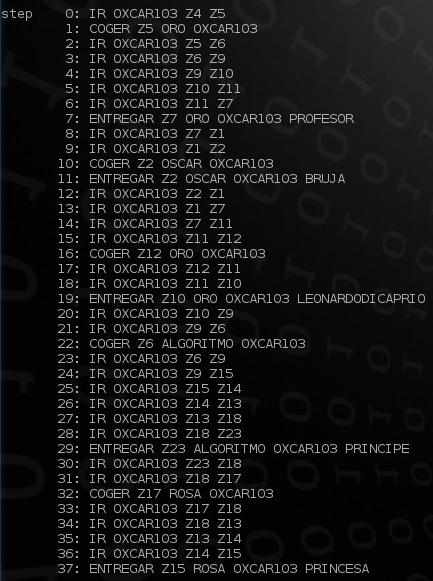
\includegraphics[width=15cm]{Problema1.jpg}
			\caption{Solución del problema 1.}
			\label{Prob-1}
		\end{figure}
		
\section{Consumo de energía}
	\subsection{Implementación}
		Para el control de la energía que le queda, haremos uso de la función \verb|(energia ?j - jugador)|
		inicializada a un cierto valor en el problema(en nuestro caso, será de 103, como cabría esperar).
		
		La única acción afectada por este cambio será \verb|ir| que debe incluir la precondición que comprueba
		la energía restante(\verb|(> (energia ?j) 0)|) y el efecto de ajustarla a su nuevo valor para futuras
		acciones(\verb|(decrease (energia ?j) 1)|).
		
	\subsection{Problema}
		La implementación del problema fue idéntica con la excepción de la inicialización de la función de
		energía al valor indicado:
		\begin{figure}[H]
			\centering
			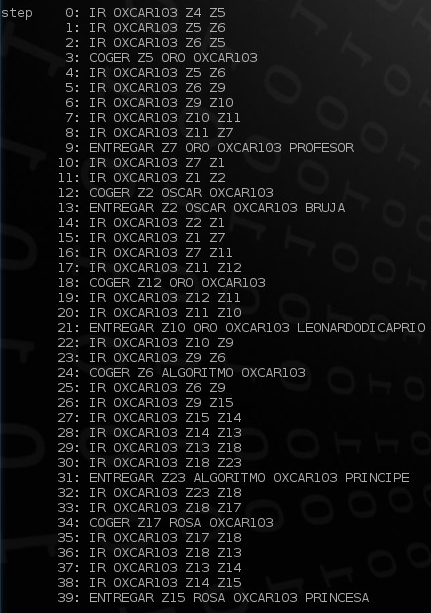
\includegraphics[width=15cm]{Problema2.jpg}
			\caption{Solución del problema 2.}
			\label{Prob-2}
		\end{figure}

\section{Tipos de terreno y mochila}
	\subsection{Desplazamiento en distintos terrenos y objetos especiales}
		La existencia de los distintos tipos de terrenos requiere de la implemetación de predicados que
		controlen el tipo de terreno del que disponemos: \verb|(esbosque ?z - zona)|, \verb|(esagua ?z - zona)|,
		\verb|(esprecipicio ?z - zona)|, \verb|(esarena ?z - zona)| y \verb|(espiedra ?z - zona)|
		
		Además, el desplazamiento por bosque o agua requiere de dos objetos especiales que también se
		controlarán por los predicados: \verb|(esbikini ?o - objeto)|, \verb|(eszapatilla ?o - objeto)|
		
		Además, debemos introducir las precondiciones de cada zona:
		\begin{itemize}
			\item Para controlar bien las condiciones de bosque y agua, he decidido separar la acción
			\verb|ir| en 3 definiciones siendo una dedicada para el bosque, otra para el agua y otra
			para el resto.
			
			\item En la acción dedicada al bosque, se comprueba lo mismo que en la acción \verb|ir| que
			teníamos previamente definida y le añadimos las condiciones de que la zona sea bosque y que
			tenemos las zapatillas:
			\begin{verbatim}
(:action ir
   :parameters (?j - jugador ?origen ?destino - zona ?o -objeto)
   :precondition (and (at ?j ?origen)
                      (> (energia ?j) 0)
                      (or
                         (conectada ?origen ?destino)
                         (conectada ?destino ?origen)
                      )
                      (esbosque ?destino)
                      (eszapatilla ?o)
                      (or
                         (cogido ?o ?j)
                         (enmochila?o ?j)
                      )
                 )
   :effect (and (at ?j ?destino)
                (not (at ?j ?origen))
                (decrease (energia ?j) 1)
           )
)
			\end{verbatim}

			\item Para la zona de agua, se procede de forma análoga salvo que la zona debe ser agua y el
			objeto, el bikini:
			\begin{verbatim}
(:action ir
   :parameters (?j - jugador ?origen ?destino - zona ?o -objeto)
   :precondition (and (at ?j ?origen)
                      (> (energia ?j) 0)
                      (or
                         (conectada ?origen ?destino)
                         (conectada ?destino ?origen)
                      )
                      (esagua ?destino)
                      (esbikini ?o)
                      (or
                         (cogido ?o ?j)
                         (enmochila?o ?j)
                      )
                 )
   :effect (and (at ?j ?destino)
                (not (at ?j ?origen))
                (decrease (energia ?j) 1)
           )
)
			\end{verbatim}

			\item Para la zona por defecto, incluimos las precondiciones de que no sea un precipio porque no puedes
			caminar por ellos, que no sea ni bosque ni agua porque para ellos están implementadas las otras opciones
			que si es piedra, le cueste más energía mediante el uso de la cláusula \textit{when}:
			\begin{verbatim}
(:action ir
   :parameters (?j - jugador ?origen ?destino - zona)
   :precondition (and (at ?j ?origen)
                      (> (energia ?j) 0)
                      (or
                         (conectada ?origen ?destino)
                         (conectada ?destino ?origen)
                      )
                      (not (esbosque ?destino))
                      (not (esagua ?destino))
                      (not (esprecipicio ?destino))
                 )
   :effect (and (at ?j ?destino)
                (not (at ?j ?origen))
                (decrease (energia ?j) 1)
                (when (espiedra ?destino) (decrease (energia ?j) 1))
           )
)
			\end{verbatim}
		\end{itemize}

	\subsection{Incorporación de mochila}
		Ahora disponemos de una mochila en la que podemos guardar un objeto, luego requiere de nuevos
		predicados que almacenen la información pertinente: \verb|(mochilalibre ?j - jugador)|,
		\verb|(enmochila ?o - objeto ?j - jugador)|
		
		También debemos incluir métodos similares a los que ya teníamos de coger y soltar objeto pero
		para meter y sacar objetos de la mochila.
		
		El método para meter objetos sería:
		\begin{verbatim}
(:action cogermochila
   :parameters (?o - objeto ?j - jugador)
   :precondition (and (manolibre ?j)
                      (enmochila ?o ?j)
                 )
   :effect (and (not (manolibre ?j))
                (mochilalibre ?j)
                (cogido ?o ?j )
                (not (enmochila ?o ?j))
           )
)
		\end{verbatim}
		
		Y su complementario sería:
		\begin{verbatim}
(:action dejarmochila
   :parameters (?o - objeto ?j - jugador)
   :precondition (and (cogido ?o ?j)
                      (mochilalibre ?j)
                 )
   :effect (and (manolibre ?j)
                (not (mochilalibre ?j))
                (not (cogido ?o ?j))
                (enmochila ?o ?j)
          )
)
		\end{verbatim}

\section{Consecución de puntos}
	\subsection{Implementación}
		Se propone ahora que cada vez que se entrega un objeto a un personaje se logre obtener una
		cuantía de puntos que se irán sumando mediante el uso de la función \verb|(puntos ?j - jugador)|
		y de la función \verb|(puntosentrega ?o - objeto ?p - personaje)| que establecerá en el archivo
		problema las puntuaciones que aportará cada objeto al entregarlo a cada personaje.
		
		La única diferencia a nivel de acciones aquí registrado es que la acción \verb|entregar|
		incorporará un efecto en el que se aplicará la suma correspondiente.
		
\section{Capacidad de la mochila}
	\subsection{Múltiples bolsillos}
		Ahora, el número de objetos que puede llevar la mochila viene dado por el archivo problema, dando
		posibilidad de no llevar ninguno y estar como en los primeros apartados o incluso poder llevar todos
		los objetos del mapa.
		
		Lo que se solucionará con dos funciones \verb|(capacidadmochila ?j - jugador)| para conocer el tope
		de la mochila y \verb|(usomochila ?j - jugador)| para el tamaño actual o equivalentemente con una
		sola función \verb|(bolsilloslibres ?j jugador)| que controla cuántos objetos aún podemos meterle.
		
		Estas nuevas funciones alteran las acciones de \textit{cogermochila} y \textit{dejarmochila}.
		
		Finalmente, \textit{cogermochila} queda así:
		\begin{verbatim}
(:action cogermochila
   :parameters (?o - objeto ?j - jugador)
   :precondition (and (manolibre ?j)
                      (enmochila ?o ?j)
                 )
   :effect (and (not (manolibre ?j))
                (decrease (usomochila ?j) 1)
                (cogido ?o ?j )
                (not (enmochila ?o ?j))
           )
)
		\end{verbatim}

		Y el método de \textit{dejarmochila} sería:
		\begin{verbatim}
(:action dejarmochila
   :parameters (?o - objeto ?j - jugador)
   :precondition (and (cogido ?o ?j)
                      (< (usomochila ?j) (capacidadmochila ?j))
                 )
   :effect (and (manolibre ?j)
                (increase (usomochila ?j) 1)
                (not (cogido ?o ?j))
                (enmochila ?o ?j)
           )
)
		\end{verbatim}
		
\section{Problemas}
	A partir del tercer problema, el programa quedaba intentando encontrar una solución y tras dejarlo
	más de una noche, opté por suprimir estos apartados por miedo a hacerle daño a mi propio portátil.
		
\end{document}
